% ============================== UNIT 4 =====================================
\unitheading{4}{Electronic configuration and periodic table}

\textit{Handout chapter 4, sections 4.1--4.2 (pages 13--15).} Three rules place the electrons of any
atom in its orbitals; the resulting configuration explains the layout of the periodic table.

\partheading{Concepts in detail}

\sect{4.1}{Electronic configuration in the ground state}
\begin{concept}[Electronic configuration.]
The list of the occupied subshells with the number of electrons in each, written as a superscript:
for example $\mathrm{O}\colon 1\mathrm s^2\,2\mathrm s^2\,2\mathrm p^4$. The superscripts add up to the number
of electrons ($Z$ for a neutral atom). The ground-state configuration follows three rules.
\end{concept}

\subsect{4.1.1\quad Aufbau (building-up) principle}
\begin{concept}[Aufbau principle.]
In the ground state, the electrons occupy the orbitals of lowest energy first. The order of the
subshells is given by Madelung's rule (Unit 3):
1s 2s 2p 3s 3p \textbf{4s 3d} 4p 5s 4d 5p 6s 4f 5d 6p 7s 5f 6d 7p.
\end{concept}

\subsect{4.1.2\quad Pauli exclusion principle (1925)}
\begin{concept}[Pauli exclusion principle.]
Two electrons of the same atom cannot have the same four quantum numbers $(n,\ell,m_\ell,m_s)$.
Consequence: one orbital (fixed $n,\ell,m_\ell$) holds \textbf{at most two electrons}, and they must
have opposite spins ($\uparrow\downarrow$, ``paired'').
\end{concept}
\begin{handout}{Table 4-1, maximum number of electrons in each subshell}
\begin{center}\small
\begin{tabular}{|l|c|c|c|c|}
\hline
Subshell & s ($\ell = 0$) & p ($\ell = 1$) & d ($\ell = 2$) & f ($\ell = 3$), for reference\\ \hline
Number of AOs ($2\ell+1$) & 1 & 3 & 5 & 7\\ \hline
Maximum number of electrons $2(2\ell+1)$ & 2 & 6 & 10 & 14\\ \hline
\end{tabular}
\end{center}
A shell $n$ holds at most $2n^2$ electrons: 2, 8, 18, 32.
\end{handout}

\subsect{4.1.3\quad Hund's rule}
\begin{concept}[Hund's rule.]
In a subshell with several orbitals (p, d, f), the electrons first occupy \emph{different} orbitals
with \emph{parallel} spins (same $m_s$) before pairing up. This configuration has the lowest energy:
electrons in different orbitals repel each other less.
\end{concept}
\begin{handout}{box after Hund's rule, example of carbon and nitrogen}
Each box is an orbital, each arrow an electron. Carbon, $1\mathrm s^2\,2\mathrm s^2\,2\mathrm p^2$, and
nitrogen, $1\mathrm s^2\,2\mathrm s^2\,2\mathrm p^3$ (2p subshell only):
\begin{center}
\begin{tabular}{l c c c}
 & \textbf{correct (Hund)} & wrong: paired too early & wrong: spins not parallel\\[2pt]
C, 2p$^2$ & \obox{u,u,e} & \obox{d,e,e} & \obox{u,w,e}\\[4pt]
N, 2p$^3$ & \obox{u,u,u} & \obox{d,u,e} & \obox{u,w,u}
\end{tabular}
\end{center}
Carbon has 2 unpaired electrons, nitrogen 3. (By convention the first electron of an orbital is drawn
$\uparrow$.) The ``wrong'' diagrams are allowed by Pauli but describe \emph{excited} states.
\end{handout}

\subsect{4.1.4\quad Mapping the first 18 elements}
Filling in order 1s, 2s, 2p, 3s, 3p and applying Pauli and Hund gives:
\begin{handout}{Table 4-2, electronic configurations from H ($Z = 1$) to Ar ($Z = 18$)}
\begin{center}\small
\renewcommand{\arraystretch}{1.35}
\begin{tabular}{|l|l|c||l|l|c|}
\hline
\multicolumn{6}{|l|}{$n = 1$ (boxes: 1s)}\\ \hline
H & $1\mathrm s^1$ & \obox{u} & He & $1\mathrm s^2$ & \obox{d}\\ \hline
\multicolumn{6}{|l|}{$n = 2$ (boxes: 2s \,|\, 2p; core [He] $= 1\mathrm s^2$)}\\ \hline
Li & $[\mathrm{He}]\,2\mathrm s^1$ & \obox{u}\;\obox{e,e,e} & Be & $[\mathrm{He}]\,2\mathrm s^2$ & \obox{d}\;\obox{e,e,e}\\ \hline
B & $[\mathrm{He}]\,2\mathrm s^2 2\mathrm p^1$ & \obox{d}\;\obox{u,e,e} & C & $[\mathrm{He}]\,2\mathrm s^2 2\mathrm p^2$ & \obox{d}\;\obox{u,u,e}\\ \hline
N & $[\mathrm{He}]\,2\mathrm s^2 2\mathrm p^3$ & \obox{d}\;\obox{u,u,u} & O & $[\mathrm{He}]\,2\mathrm s^2 2\mathrm p^4$ & \obox{d}\;\obox{d,u,u}\\ \hline
F & $[\mathrm{He}]\,2\mathrm s^2 2\mathrm p^5$ & \obox{d}\;\obox{d,d,u} & Ne & $[\mathrm{He}]\,2\mathrm s^2 2\mathrm p^6$ & \obox{d}\;\obox{d,d,d}\\ \hline
\multicolumn{6}{|l|}{$n = 3$ (boxes: 3s \,|\, 3p; core [Ne] $= 1\mathrm s^2 2\mathrm s^2 2\mathrm p^6$)}\\ \hline
Na & $[\mathrm{Ne}]\,3\mathrm s^1$ & \obox{u}\;\obox{e,e,e} & Mg & $[\mathrm{Ne}]\,3\mathrm s^2$ & \obox{d}\;\obox{e,e,e}\\ \hline
Al & $[\mathrm{Ne}]\,3\mathrm s^2 3\mathrm p^1$ & \obox{d}\;\obox{u,e,e} & Si & $[\mathrm{Ne}]\,3\mathrm s^2 3\mathrm p^2$ & \obox{d}\;\obox{u,u,e}\\ \hline
P & $[\mathrm{Ne}]\,3\mathrm s^2 3\mathrm p^3$ & \obox{d}\;\obox{u,u,u} & S & $[\mathrm{Ne}]\,3\mathrm s^2 3\mathrm p^4$ & \obox{d}\;\obox{d,u,u}\\ \hline
Cl & $[\mathrm{Ne}]\,3\mathrm s^2 3\mathrm p^5$ & \obox{d}\;\obox{d,d,u} & Ar & $[\mathrm{Ne}]\,3\mathrm s^2 3\mathrm p^6$ & \obox{d}\;\obox{d,d,d}\\ \hline
\end{tabular}
\end{center}
The full form of Cl, for example, is $1\mathrm s^2\,2\mathrm s^2\,2\mathrm p^6\,3\mathrm s^2\,3\mathrm p^5$.
The shorthand writes the previous noble gas in brackets for the core.
\end{handout}
\begin{worked}[: iron, $Z = 26$]
Fill in Madelung order: $1\mathrm s^2\,2\mathrm s^2\,2\mathrm p^6\,3\mathrm s^2\,3\mathrm p^6$ (18
electrons, [Ar]), then $4\mathrm s^2$ (20), then 6 electrons in 3d (26):
$\mathrm{Fe}\colon [\mathrm{Ar}]\,4\mathrm s^2\,3\mathrm d^6$, often written $[\mathrm{Ar}]\,3\mathrm d^6\,4\mathrm s^2$
(by increasing $n$), as on the handout's periodic table. 3d boxes: \obox{d,u,u,u,u}: 4 unpaired electrons.
\end{worked}

\subsect{4.1.5\quad Core and valence electrons}
\begin{concept}[Core electrons.]
Electrons in the low-energy AOs, close to the nucleus and strongly bound. They take no part in
chemistry. They make up the configuration of the previous noble gas, written in brackets.
\end{concept}
\begin{concept}[Valence electrons.]
Electrons in the highest-energy AOs, far from the nucleus and weakly bound: those of the highest $n$,
plus those of an unfilled $(n-1)$d subshell for transition metals. They determine the chemical
properties. They are the electrons written after the bracket.
\end{concept}
Example: Cl $= [\mathrm{Ne}]\,3\mathrm s^2\,3\mathrm p^5$ has 10 core electrons and 7 valence electrons.
It needs one electron to reach the configuration of argon, which is why it forms $\ce{Cl-}$.
\begin{concept}[Configurations of ions.]
Anions: add electrons in the next free orbitals ($\ce{Cl-}\colon [\mathrm{Ne}]\,3\mathrm s^2 3\mathrm p^6 =
[\mathrm{Ar}]$). Cations: remove electrons from the \emph{highest} $n$ first. For transition metals the
4s electrons leave before the 3d ones: $\ce{Fe^2+}\colon [\mathrm{Ar}]\,3\mathrm d^6$,
$\ce{Fe^3+}\colon [\mathrm{Ar}]\,3\mathrm d^5$ (not $[\mathrm{Ar}]\,4\mathrm s^2\,3\mathrm d^3$).
\end{concept}

\sect{4.2}{The periodic table of the elements}
\subsect{4.2.1\quad Structure}
\begin{itemize}
  \item Elements are placed in order of increasing \textbf{atomic number $Z$}.
  \item \textbf{18 columns = groups}: elements of a group have the same valence configuration and similar
        chemistry (group 1: alkali metals, 2: alkaline-earth metals, 17: halogens, 18: noble gases).
  \item \textbf{7 rows = periods}: period $n$ is the filling of the valence shell $n$ (it starts with
        $n$s$^1$ and ends with $n$p$^6$, except period 1).
  \item \textbf{Blocks} named after the subshell being filled: s (groups 1--2, and He), p (13--18),
        d (3--12, transition metals), f (lanthanides and actinides, drawn below).
  \item \textbf{Mendeleev} (1869) ordered the known elements by atomic \emph{mass} and grouped them by
        properties, leaving gaps for undiscovered elements (gallium, germanium) whose properties he
        predicted. Today the order is by $Z$, which also fixes the few inversions of mass (Ar/K, Co/Ni, Te/I).
\end{itemize}
\begin{center}
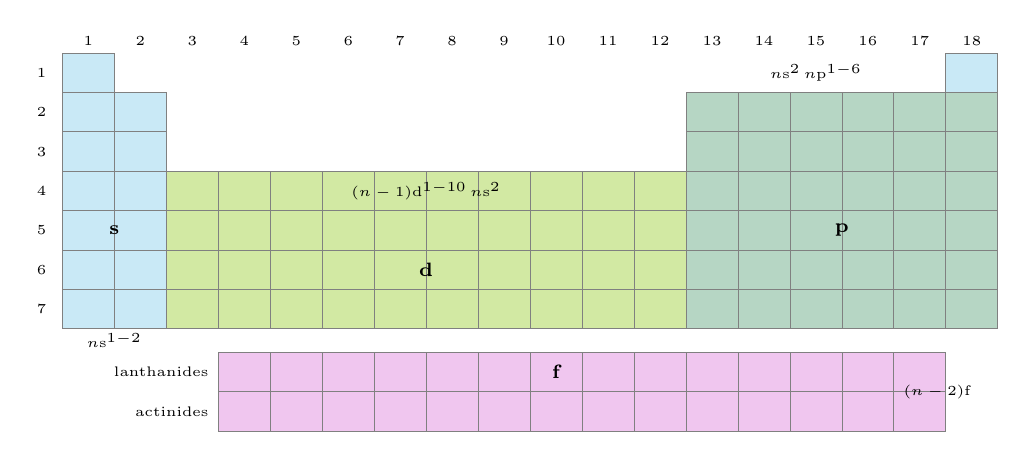
\begin{tikzpicture}[x=0.66cm, y=0.5cm]
  \tikzset{cell/.style={draw=black!50, line width=0.3pt}}
  % s block
  \foreach \p in {1,...,7} \fill[cell, fill=SkyBlue!45] (0,-\p) rectangle ++(1,1);
  \foreach \p in {2,...,7} \fill[cell, fill=SkyBlue!45] (1,-\p) rectangle ++(1,1);
  \fill[cell, fill=SkyBlue!45] (17,-1) rectangle ++(1,1);
  % d block
  \foreach \p in {4,...,7} \foreach \g in {2,...,11} \fill[cell, fill=YellowGreen!45] (\g,-\p) rectangle ++(1,1);
  % p block
  \foreach \p in {2,...,7} \foreach \g in {12,...,17} \fill[cell, fill=SeaGreen!35] (\g,-\p) rectangle ++(1,1);
  % f block
  \foreach \r in {9,10} \foreach \g in {3,...,16} \fill[cell, fill=Orchid!40] (\g,-\r+0.4) rectangle ++(1,1);
  \foreach \g in {1,...,18} \node[font=\tiny] at (\g-0.5,0.3) {\g};
  \foreach \p in {1,...,7} \node[font=\tiny] at (-0.4,-\p+0.5) {\p};
  \node[font=\scriptsize\bfseries] at (1,-4.5) {s};
  \node[font=\scriptsize\bfseries] at (7,-5.5) {d};
  \node[font=\scriptsize\bfseries] at (15,-4.5) {p};
  \node[font=\scriptsize\bfseries] at (9.5,-8.1) {f};
  \node[font=\tiny] at (1,-7.3) {$n\mathrm s^{1-2}$};
  \node[font=\tiny] at (7,-3.5) {$(n-1)\mathrm d^{1-10}\,n\mathrm s^2$};
  \node[font=\tiny] at (14.5,-0.5) {$n\mathrm s^2\,n\mathrm p^{1-6}$};
  \node[font=\tiny, anchor=east] at (3,-8.1) {lanthanides};
  \node[font=\tiny, anchor=east] at (3,-9.1) {actinides};
  \node[font=\tiny, anchor=west] at (16,-8.6) {$(n-2)\mathrm f$};
\end{tikzpicture}
\end{center}
The length of the periods follows from Madelung's order: period 1 fills 1s (2 elements); periods 2
and 3 fill $n$s and $n$p (8); periods 4 and 5 fill $n$s, $(n-1)$d, $n$p (18); periods 6 and 7 also
fill $(n-2)$f (32).

\subsect{4.2.2\quad Valence configuration from the position in the table}
\begin{itemize}
  \item Period number $=$ largest $n$ of the configuration.
  \item s and p blocks: number of valence electrons = the position in the period (group 1: 1, group 2:
        2, groups 13--18: 3 to 8). Example: sulfur, period 3, group 16: 6 valence electrons,
        $[\mathrm{Ne}]\,3\mathrm s^2 3\mathrm p^4$.
  \item d block: valence configuration $(n-1)\mathrm d^{x}\,n\mathrm s^2$ with $x = $ group $- 2$.
        Example: manganese, period 4, group 7: $[\mathrm{Ar}]\,3\mathrm d^5\,4\mathrm s^2$.
  \item Elements of the same group have the same valence configuration with a different $n$:
        Li $2\mathrm s^1$, Na $3\mathrm s^1$, K $4\mathrm s^1$ \dots
\end{itemize}
\begin{concept}[Exceptions to Madelung's rule.]
The rule is always followed in the s and p blocks, but not always in the d and f blocks, where the $n$s
and $(n-1)$d levels are very close. A half-filled or filled d subshell is especially stable:
\begin{center}
Cr: $[\mathrm{Ar}]\,3\mathrm d^5\,4\mathrm s^1$ (not $3\mathrm d^4 4\mathrm s^2$)\qquad
Cu: $[\mathrm{Ar}]\,3\mathrm d^{10}\,4\mathrm s^1$ (not $3\mathrm d^9 4\mathrm s^2$).
\end{center}
The same happens for Mo, Ag and Au below them.
\end{concept}
\begin{trap}
Count electrons, not protons, for an ion. When writing a cation of a transition metal, remove 4s
before 3d. Do not confuse the group number (1--18) with the number of valence electrons in the d block:
Fe is in group 8 and has 8 valence electrons ($3\mathrm d^6\,4\mathrm s^2$), but in the p block chlorine
is in group 17 and has 7.
\end{trap}

% ------------------------------------------------------------------ recap
\clearpage
\begin{recap}{Unit 4: electronic configuration and periodic table}
\recapsub{The three filling rules}
\textbf{Aufbau}: lowest-energy orbitals first, in Madelung order
1s 2s 2p 3s 3p 4s 3d 4p 5s 4d 5p 6s 4f 5d 6p 7s.\\
\textbf{Pauli}: no two electrons with the same $(n,\ell,m_\ell,m_s)$: at most 2 electrons per orbital,
with opposite spins.\\
\textbf{Hund}: in a subshell, fill every orbital singly with parallel spins before pairing.

\recapsub{Capacities}
s: 1 AO, 2 e$^-$;\quad p: 3 AOs, 6 e$^-$;\quad d: 5 AOs, 10 e$^-$;\quad f: 7 AOs, 14 e$^-$;\quad
shell $n$: $2n^2$ e$^-$.

\recapsub{Method for a configuration}
(1) Count the electrons ($Z$, minus the charge). (2) Fill in Madelung order. (3) Replace the core by
the previous noble gas in brackets. (4) Draw boxes for the valence subshells using Pauli and Hund; count
unpaired electrons. (5) Cations of d-block metals: remove $n$s first.

\recapsub{Periodic table}
Order by $Z$;\ 18 groups (same valence configuration, similar chemistry);\ 7 periods (period
number = valence shell $n$);\ blocks s, p, d, f = subshell being filled. Period lengths 2, 8, 8, 18,
18, 32, 32. Valence configuration: s block $n\mathrm s^{1-2}$, p block $n\mathrm s^2 n\mathrm p^{1-6}$,
d block $(n-1)\mathrm d^{1-10} n\mathrm s^{2}$.

\recapsub{Key examples}
O $[\mathrm{He}]2\mathrm s^2 2\mathrm p^4$ (2 unpaired);\ Cl $[\mathrm{Ne}]3\mathrm s^2 3\mathrm p^5$
(7 valence e$^-$);\ Fe $[\mathrm{Ar}]3\mathrm d^6 4\mathrm s^2$;\ $\ce{Fe^3+}$ $[\mathrm{Ar}]3\mathrm d^5$;\
Cr $[\mathrm{Ar}]3\mathrm d^5 4\mathrm s^1$;\ Cu $[\mathrm{Ar}]3\mathrm d^{10} 4\mathrm s^1$.

\recapsub{You should be able to}
\begin{itemize}
  \item write the ground-state configuration (full and shorthand) of any atom or ion up to $Z = 36$;
  \item draw box diagrams and count unpaired electrons;
  \item find the period, group and block from a configuration, and the reverse;
  \item separate core and valence electrons;
  \item recognise ground, excited and impossible configurations.
\end{itemize}
\end{recap}
